\selectlanguage{english}%

\chapter{Experiment set-up and detectors}


\section{The Relativistic Heavy Ion Collider}

The Relativistic Heavy Ion Collider (RHIC) at Brookhaven Nation Laboratory
(BNL) was built at year 1999, after nine years construction. It is
deigned to accelerate and collide heavy ions and polarized protons
at relativistic energy. RHIC has capabilities to deliver beams ranged
from proton to uranium with high luminosity. The top center-of-mass
collision energy is 200 GeV per nucleon pair for heavy ion collisions
and 500 GeV for polarized p+p collisions. The basic design parameters
of the collider are listed in Table \ref{table: RHIC parameters}.
The main physics goal of RHIC is to investigate the phase transition
from hadronic phase to QGP phase and to study the formation and property
of QGP. RHIC also provides polarized p+p collision with collision
energy up to 500 GeV to expand the scientific objective of RHIC to
include vigorous spin physics program.

Figure \ref{fig:RHIC overview} shows the layout of RHIC complex with
the injector chain and the ring tunnel. The RHIC complex contains
the Tandem van de Graaff pre-accelerator, a linear proton accelerator,
the Booster Synchrotron, the Alternating Gradient Synchrotron (AGS)
and and ultimately the RHIC synchrotron ring. The acceleration scenario
for gold ion beams is shown in Fig. \ref{fig: ASfor Au}. Negatively
charged ($Q_{T}=-1$) Au ions is injected into the Tandem Van de Graaff
from the Pulsed Sputter Ion Source. They are partially stripped of
their electrons and accelerated inside the Tandem Van de Graaff and
exit with the energy of 1 MeV/nucleon and charge state of $Q_{T}=+32$.
The ions are delivered to the Booster Synchrotron and accelerated
to 95 MeV/nucleon and further stripped to $Q_{T}=+77$ at the exit.
Then they are transferred into the AGS, where they are accelerated
to 8.86 GeV/nucleon and sorted into four final bunches. Ions are fully
stripped ($Q_{T}=+79$) at the exit of the AGS and transported to
the RHIC storage rings though the AtR beamline. RHIC also has capability
to provide polarized proton beams. Protons are injected from the 200
MeV Linac into the booster, followed by acceleration in the AGS and
injection into RHIC.

RHIC has two concentric super-conducting accelerator/storage rings,
one (``Blue Ring'') for clockwise and the other (``Yellow Ring'')
for anti-clockwise beams. They are on a common horizontal plane in
the tunnel with a circumference about 38 km. Each ring consists of
six insertion sections with collision point at their center along
its circumference. Two major experiments STAR and PHENIX are located
at 6 o'clock and 8 o'clock, and two minor ones PHOBOS and BRAHMS were
located at 10 o'clock and 2 o'clock, respectively. To date, RHIC has
been configured to run in p+p, d+Au, Au+Au, Cu+Cu, Cu+Au and U+U collisions.

\begin{table}
\begin{centering}
\begin{tabular}{ccc}
\hline 
 & For Au+Au & For p+p\tabularnewline
\hline 
\hline 
Beam energy & $\rightarrow$100 GeV/nucleon & 30$\rightarrow$250 GeV\tabularnewline
Luminosity & $2\times10^{26}cm^{-2}s^{-1}$ & $1.4\times10^{31}cm^{-2}s^{-1}$\tabularnewline
Number of Bunches/ring & 60($\rightarrow$120) & 60($\rightarrow$120)\tabularnewline
Luminosity lifetime & \textasciitilde{} 10 hours & \textasciitilde{} 10 hoours\tabularnewline
\hline 
\end{tabular}
\par\end{centering}

\protect\caption{Performance specifications of RHIC \cite{Adler2003433}.}


\label{table: RHIC parameters}
\end{table}
 

\begin{figure}
\begin{centering}
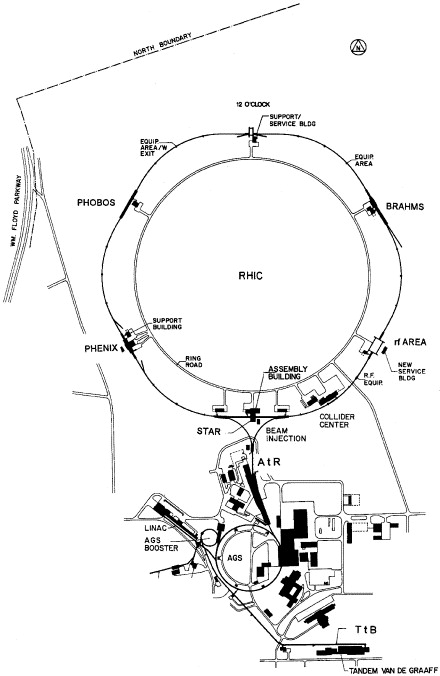
\includegraphics[width=0.6\textwidth]{fig/2.Detector/RHIC_overview}
\par\end{centering}

\protect\caption{The layout of RHIC complex\cite{Hahn2003245}.}


\label{fig:RHIC overview}
\end{figure}


\begin{figure}
\begin{centering}
\includegraphics[width=0.6\textwidth]{\string"fig/2.Detector/RHIC Au+Au\string".png}
\par\end{centering}

\protect\caption{Acceleration scenario for gold ions\cite{Adler2003433}.}


\label{fig: ASfor Au}
\end{figure}



\section{STAR experiment}

The Solenoidal Tracker at RHIC (STAR) is one of the two large detecter
systems constructed at RHIC. Heavy ion collision at RHIC creates a
nuclear environment of a large produced particles (up to approximately
1000 per unit pseudo-rapidity) and high momentum particles from hard
parton-parton scattering. The main physics goal of the STAR experiment
is to measure many observables simultaneously to investigate the signatures
of a possible QGP phase transition and to understand the space-time
evolution of the collision process in ultra-relativistic heavy ion
collisions. In order to accomplish this, STAR was designed primarily
for measurements of hadron production over a large solid angle. The
STAR detector systems are very effective in high precision tracking,
momentum analysis, and particle identification at the central rapidity
region. With the installation of the Time Of Flight detector (TOF)
in 2009, STAR gained the capability to identify electrons and positions.

STAR has an azimuthal symmetric acceptance and covers large range
around mid-rapidity ($|\eta|$<1, $2\pi$ azimuthal coverage). Figure
\ref{fig: STAR det} shows the layout of the STAR detector systems
alone with the subsystems. 

Close to the beam pipe is the Heavy Flavor Tracker (HFT) which is
a new detector add in the STAR detector systems in 2014. The HFT is
designed to measure the heavy flavor production by the measurement
of displaced vertices and to do the direct topological identification
of open charm hadrons. The Time Projection Chamber (TPC) is the main
tracker at STAR which has a coverage of $|\eta|$<1 and $2\pi$ in
azimuthal direction. The Time Of Flight (TOF) detector is surrounding
the TPC which has also a coverage $|\eta|$<1 and $2\pi$ in azimuthal
direction. The Barrel Electro-Magnetic Calorimeter (BEMC) located
outside of the TOF and covers $|\eta|<1$ with complete azimuthal
symmetry. The Endcap Electro-Magnetic Calorimeter (EEMC) covers for
1 < |η| < 2, over the full azimuthal range. The EMCs are used to distinguish
high momentum single photons from photon pairs of π and η meson decays
and electrons from charged hadrons. Outside the BEMC is the magnet
system which provides a uniform magnetic field parallel to the beam
direction and together with BEMC it also servers as the electron and
hadron absorber for the Muon Telescope Detector (MTD). The MTD is
also a new added detector, which is installed in 2014. It is designed
to detect high $p_{T}$ muon for heavy flavor collectivity and production. 

Along the beam pipe, there are some trigger detectors: Zero Degree
Calorimeter (ZDC), Vertex Position Detector (VPD) and Beam-Beam Counter
(BBC). Two ZDCs locates on each side \textasciitilde{} 18 m away from
the collision point. The ZDCs are designed as hadronic calorimeters
to detect the outgoing neutrons. Dipole magnets are put before the
ZDC detectors to bend away the charged fragments. The ZDC signals
are used for monitoring the heavy ion beam luminosity and for the
experiments triggers. The BBC subsystem covers $3.3<|\eta|<5.0$ and
consists of two disk shaped scintillating detectors. They are placed
at the endcaps of the TPC (3.5 m from TPC center). Each BBC disk is
made up of close packed hexagonal scintillator tiles in two rings.
A BBC trigger corresponds to a prompt coincidence between at least
one (out of eighteen total) tile firing in both BBC EAST and BBC WEST
within a time window. This BBC trigger defines a minimum bias trigger
corresponding to a p-p cross section of $\thickapprox$ 26 mb, 87\%
of the p-p Non-Singly Diffractive (NSD) inelastic cross section. The
VPD detector has two assembly which consists of two rings of readout
detectors (19 channels). The two assemblies are mounted symmetrically
with respect to the center of STAR at a distance of 5.7 m and cover
$4.24\le\eta\le5.1$. The signals from VPD are used to select minimum
bias collisions, to constrain the location of the primary collision
vertex along the beam pipe and to provide start time for STAR fast
timing detectors. EMCs is also used to trigger on high $p_{T}$ particle
events.

The detectors involved in this analysis will be introduced in detail
in follow sections. 

\begin{figure}
\begin{centering}
\includegraphics[width=0.8\textwidth]{\string"fig/2.Detector/STAR det\string".png}
\par\end{centering}

\protect\caption{The STAR detectors. HFT and MTD are new added detectors and were fully
installed in 2014.}


\label{fig: STAR det}
\end{figure}



\subsection{STAR magnet system}

The STAR magnet system \cite{Ackermann2003624} is a room temperature
solenoidal magnet which was designed as a cylinder with a length of
6.85 m and has inner and outer diameter of 5.27 m and 7.32 m, respectively.
It provides an uniform magnetic field which parallels to the beam
direction (Z direction) with a maximum value 0.5 T for charged particle
momentum analysis. STAR magnet can work under full field (+0.5 T),
reversed full field (-0.5 T) and half field configuration ($\pm$0.25
T).


\subsection{Main tracker - Time Projection Chamber}

The Time Projection Chamber (TPC) is the primary tracking detector
and the heart of STAR detector system. The TPC was designed to record
the tracks of particles, measure their momenta, and provide particle
identification by measuring their ionization energy loss (\emph{dE/dx}).
It has a large acceptance around middle rapidity ($|\eta|<1.8$ )
and full azimuthal coverage. 

Figure \ref{fig:TPC} shows the STAR TPC. It was built as a cylinder
with a length of 4.2 m and outer diameter of 4 m and inner diameter
of 1 m. TPC was installed inside the STAR magnet system which provides
a 0.5 T uniform magnetic field. The beam pipe which is alone the Z
direction goes through the center axis of TPC and concentric with
TPC. The collisions happens in side the beam pipe near the center
of TPC.

Inside the TPC, it is an empty volume which is filled with P10 gas
(10\% methane, 90\% argon) regulated at 2 mbar above atmospheric pressure.
There is a well defined, uniform, electric field of $\thickapprox$135
V/cm in the volume serve as the drift field. The primary advantage
of P10 gas is that electrons has a fast drift velocity which peaks
at a low electric field which makes the drift velocity stable and
insensitive to small changes in temperature and pressure. The uniform
drift field in TPC is defined by a thin conductive Central Membrane
(CM) at the center of the TPC, concentric field-cage cylinders and
the readout end caps \cite{Anderson2003659}. The central membrane
is operated at 28 kV and the end caps are at ground. The typical drift
velocity of electrons in the STAR TPC is 5.45 cm/$\mu s$. The transverse
diffusion is 230 $\mu m/\sqrt{cm}$ and the longitudinal diffusion
is 360 $\mu m/\sqrt{cm}$ with 140V/cm drift field and 0.5 T magnetic
field. 

The STAR TPC's readout system is based on Multi-Wire Proportional
Chambers (MWPC) with readout pads. The readout planes are arranged
as on a clock with 12 sectors around the circle at each end of TPC.
The readout system includes four components: a pad plane and three
wire planes, shown in Fig. \ref{fig:outer_wires}. The anode wire
plane of 20 $\mu m$ wires with the pad plane on one side and the
ground wire plane on the other composes the amplification readout
layer. It can provide an amplification of 1000 to 3000 while the drifting
electrons avalanche in the high fields. Figure \ref{fig:pad_plane}
shows the anode pad plane with one full sector. To optimize the \emph{dE/dx
}resolution, the outer sector was designed to have continuous pad
coverage. This setup can improve statistics on the \emph{dE/dx }measurement
because the full track ionization signal is collected with more ionization
electrons. The inner sub sectors are in the region of highest track
density. The design of inner pads is optimized for good two-hit resolution
by using smaller pads with separate pad rows instead of continuous
pad coverage. The third wire plane is a gating grid which is a gate
to control electrons from TPC drift volume to MWPC. It also stops
the positive ions inside MWPC from entering the drift volume to preserve
the uniform drift field \cite{Anderson2003679}.

When the charged particles travel through the gas volume, they liberate
electrons from the gas molecules due to ionization energy loss. The
released secondary electrons drift under the drift field to the ends
of TPC and collected by the readout system. The signals then are digitalized
and transmitted to STAR Data AcQuistion system (DAQ). These raw signals
(ADC and TDC) are reconstructed into 3D position informations of the
ionization (hit positions) by a Kalman filte with a typical resolution
0.5\textasciitilde{}1.0 mm. The tracks of particles are reconstructed
with high precision from these hits informations in 3 dimension by
Time Projection chamber Tracker (TPT) algorithm. These tracks are
combined with other available tracking detector's results and refit
by a Kalman filter routine. Then the primary collision vertex is reconstructed
from these global tracks. The primary vertex resolution is \textasciitilde{}
350 μm with more than 1000 tracks. Furthermore, tracks with the \emph{distance
of closest approach} (dca) to the primary vertex less then 3 cm is
refitted by forcing the track to originate from the primary vertex,
these tracks are called primary tracks which has improved resolution
in position and momentum due to the relatively high precision of primary
vertex. The reconstruction efficiency including the detector acceptance
for primary tracks depends on the particle type, track quality cuts,
$p_{T}$, track multiplicity etc. The typical value for the primary
pions with $N_{fit}$ > 24 and |$\eta$| < 0.7, dca < 3.0 cm is approximate
constant at $p_{T}$ > 0.4 GeV/c: $>\sim$ 90\% for Au + Au peripheral
collisions and \textasciitilde{} 80\% for central collisions, respectively.

With the collected ionization energy loss (\emph{dE/dx}) information,
TPC also provides capability for particle identification. The mean
rate of \emph{dE/dx }is given by the Bethe-Bloch equation \ref{eq: Bethe-Bloch}
\cite{Eidelman20041}:

\begin{equation}
-\frac{dE}{dx}=Kz^{2}\frac{Z}{A}\frac{1}{\beta^{2}}\left[\frac{1}{2}\ln\frac{2m_{e}c^{2}\beta^{2}\gamma^{2}T_{max}}{I^{2}}-\beta^{2}-\frac{\delta}{2}\right]\label{eq: Bethe-Bloch}
\end{equation}
and furthermore optimized by the Bichsel functions \cite{Bichsel2006154}.
For each track, \emph{dE/dx }is extracted from the deposit charge
collected on the pad rows up to 45. Energy loss of a charged particle
for a given track length can be described by the Bichsel function
\cite{Bichsel2006154}. However, the mean of the distribution is sensitive
to the fluctuations in the tail of the distribution. Therefore, the
most probable \emph{dE/dx} is measured by removing the highest 30\%
of the measured clusters. Figure \ref{fig:dEdx_Bichsel} shows the
70\% truncated mean dE/dx distribution as well as the expectation
from Bichsel functions. Clearly the energy loss is different corresponding
to different particle species at the same momentum. In Au+Au 200 GeV
collision, STAR can separate $\pi$ and $K$ up to \textasciitilde{}
0.7 GeV/c and identify proton up to \textasciitilde{} 1.1 GeV/c.

\textbf{\emph{dE/dx}}\textbf{ calibration} is performed for each run
setups respect to collision type, collision energy and magnetic field.
The calibration is done with a specified data sample selected by following
requirement:
\begin{itemize}
\item Good clusters : used in track fit, without overlaps.
\item Good global tracks : with track length in TPC > 20 (or 40) cm.
\item Tracks with 0.4 < p < 0.5 GeV/c (\textasciitilde{}MIP for pions: $\beta\gamma=p/m=4$)
where $\pi$ can be well separated from other particles and the $\beta\gamma$
dependence of \emph{dE/dx }is completely defined by Bichsel model.
\end{itemize}
The $dE/dx$ calibration process contains a lot of corrections due
to the energy loss in TPC is influenced by many factors, but usually
it can be separated into three step: a over all correction of gas
gains for sectors and rows; correction for gas pressure dependence;
correction of track length. A value \emph{Z }is defined as flowing:

\begin{equation}
Z_{\pi}=log\left(\frac{dE/dx_{measure}}{dE/dx_{Bichsel}^{\pi}}\right)\label{eq:Zpi}
\end{equation}
Where $dE/dx_{Bichsel}^{\pi}$ is the predicted for $\pi$ from Bichsel
model. The \emph{$Z_{\pi}$ }distributions are parameterized by a
5 gaussians fit with respect to mean position ($\mu$) and width ($\sigma$)
of $\pi$, which contain contribution from $\pi$, $K$, $p$, $d$
and $e$. The relative positions of other particles to $\pi$ are
fixed. And the position ($\mu$) of $\pi$ defines the calibration
correction. The correction parameters are defined which provide condition:
$\mu=0$ and variation is within 1\% level. Figure \ref{fig:SecRow_24_40}
shows an example of the 5 gaussians fit for sector 24 row 40 in Run11
p+p 500 GeV collisions. The calibration is separated into 4 passes:
\begin{enumerate}
\item pass 0: Gas gain correction for sector/row. The $Z_{\pi}$ distributions
are parameterized in each sector and row. The correction is defined
to direction shift $\mu$ to 0 for each sector and row which generates
a correction table. Figure \ref{fig:SecRowCor} shows the variation
vs Sector and Row before correction (before) and after correction
(after).
\item pass 1: Dependence of gas gain on gas density due to pressure. Figure
\ref{fig:PresureCor} shows the $dE/dx$ variation vs gas pressure
before and after the correction. A linear fit is used to parameterize
pressure dependence of $dE/dx$ variation and to define the correction.
\item pass 2: Dependence of the truncated mean for track's \emph{dE/dx}
and its relative error versus track length in TPC. Figure \ref{fig:TrackLengthCor}
shows the track length dependence before correction and after correction.
Usually a polynomial function is used to define the correction.
\item pass 3: Final pass to check the calibration results.
\end{enumerate}
The corrections are not independent with each other, so after each
new pass, the results for previous correction need to be checked.
If the variation is larger than 1\%, another pass is need to redone
previous correction. Figure \ref{fig:dEdx_Calib_procedure} shows
the procedure of \emph{dE/dx }calibration. The requirement for dE/dx
resolution achievable with our calibration procedure has been set
as 7.5\% for tracks with length in TPC equal to 76.2 cm. Here take
the calibration for p+p 500GeV in Run11 as an example, without any
correction the \emph{dE/dx} resolution for tracks with 76.3 cm length
in TPC is 7.73\% and the one with all corrections is 6.82\% (Fig \ref{fig:dEdxRes}).

\begin{figure}
\begin{centering}
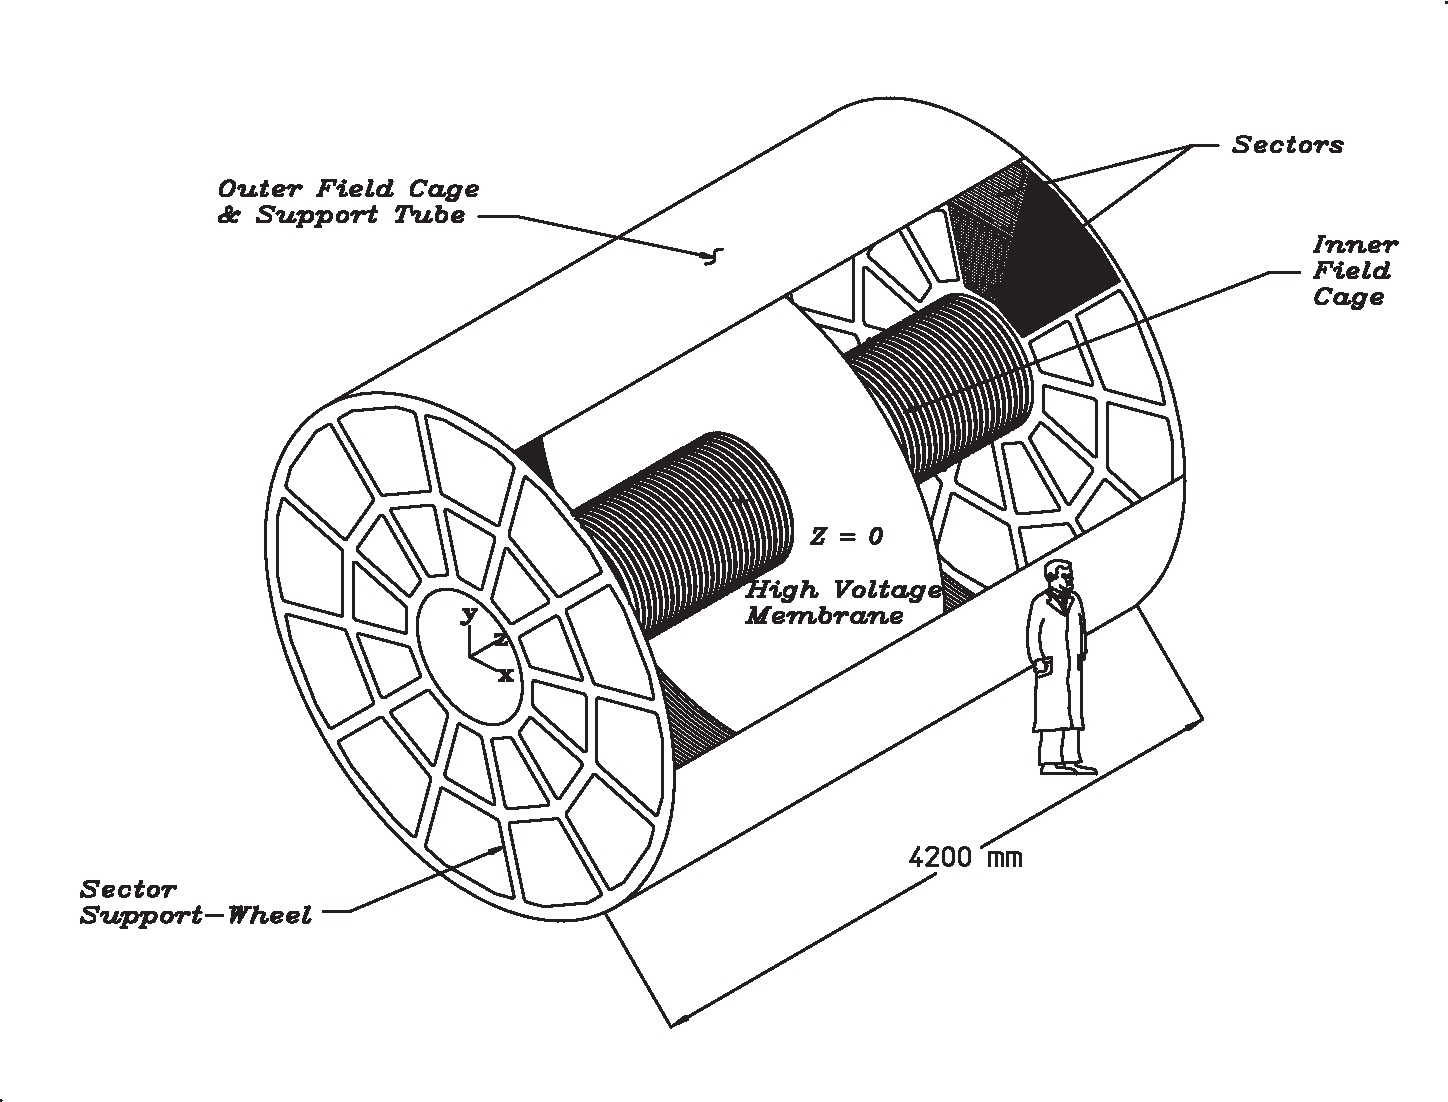
\includegraphics[width=0.8\textwidth]{fig/2.Detector/TPC/tpcman}
\par\end{centering}

\protect\caption{The STAR Time Projection Chamber (TPC) \cite{Anderson2003659}.}


\label{fig:TPC}
\end{figure}
 

\begin{figure}
\begin{centering}
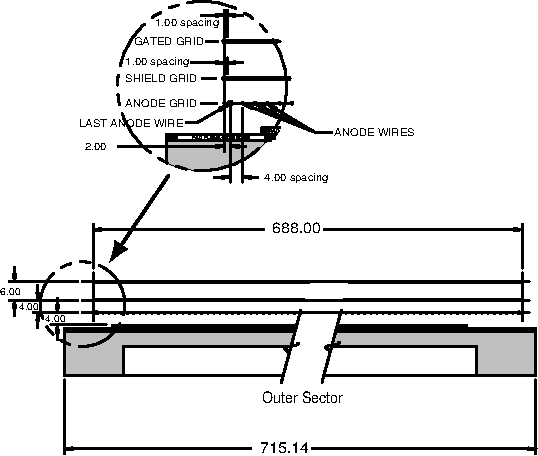
\includegraphics[width=0.8\textwidth]{fig/2.Detector/TPC/outer_wires}
\par\end{centering}

\protect\caption{}


\label{fig:outer_wires}
\end{figure}


\begin{figure}
\begin{centering}
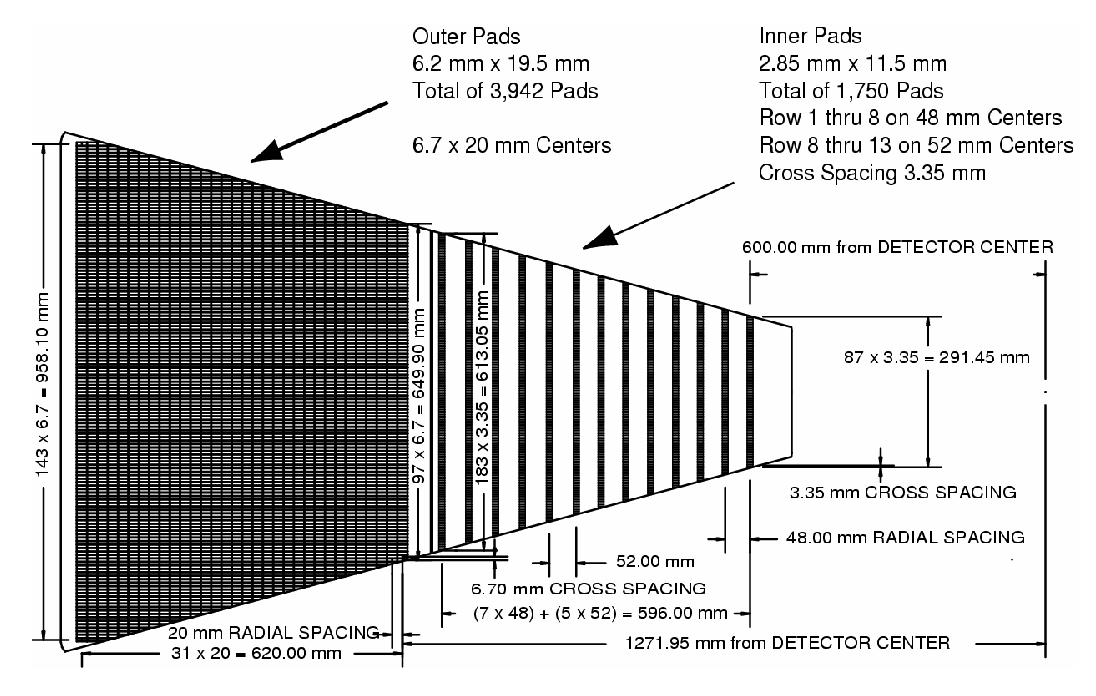
\includegraphics[width=0.8\textwidth]{/Users/luthien/Documents/Thesis/GitServer/Thesis/fig/2.Detector/TPC/padplane}
\par\end{centering}

\protect\caption{The anode pad plane with one full sector.}


\label{fig:pad_plane}
\end{figure}


\begin{figure}
\begin{centering}
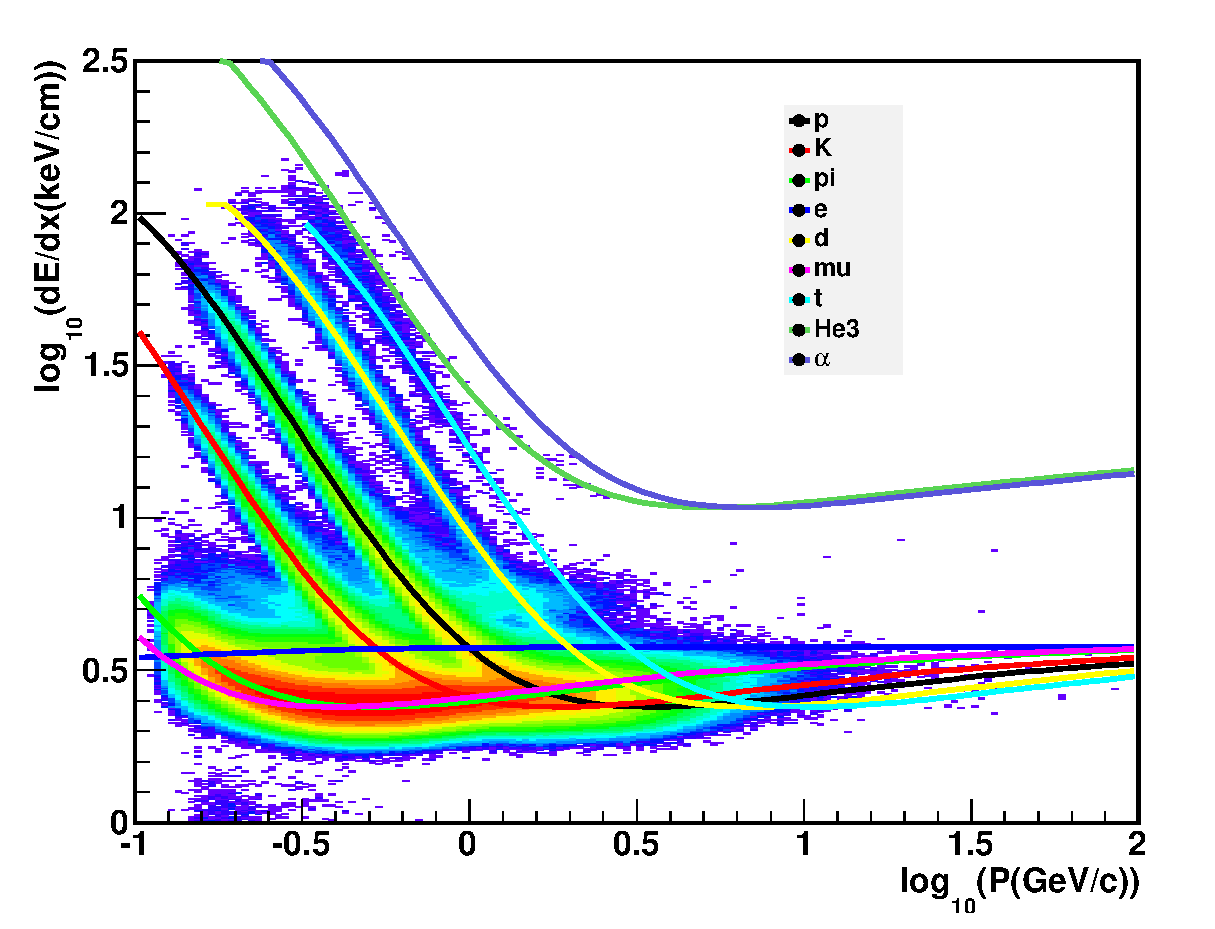
\includegraphics[width=0.8\textwidth]{fig/2.Detector/TPC/dEdx}
\par\end{centering}

\protect\caption{Distribution of \emph{dE/dx} as a function of momentum. The Bishcel
functions are also shown for difference particle species.}


\label{fig:dEdx_Bichsel}
\end{figure}


\begin{figure}
\begin{centering}
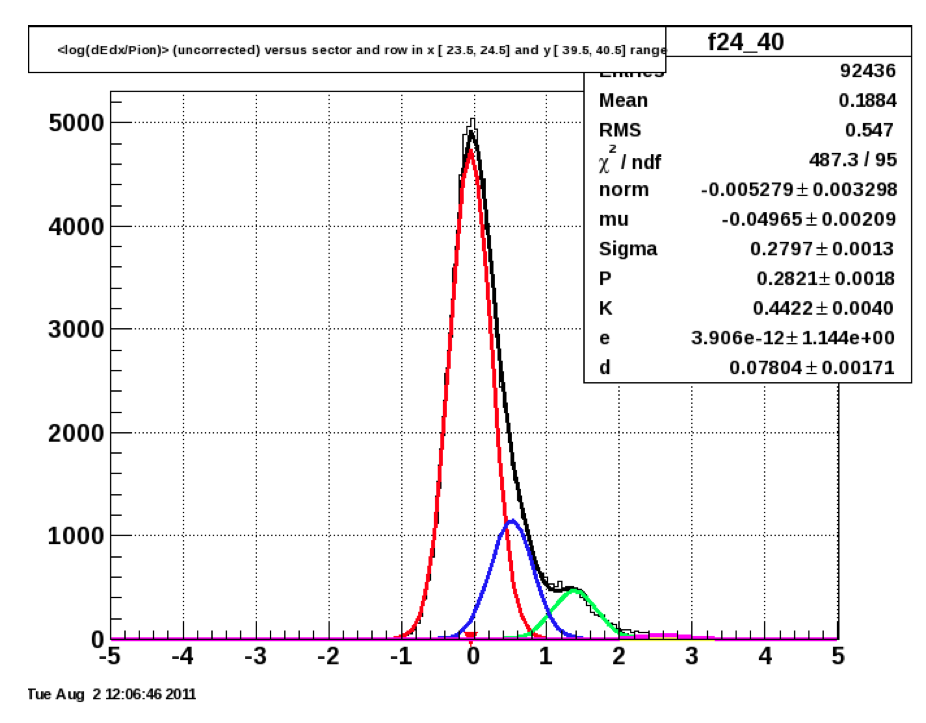
\includegraphics[width=0.8\textwidth]{/Users/luthien/Documents/Thesis/GitServer/Thesis/fig/2.Detector/TPC/SecRow_24_40}
\par\end{centering}

\protect\caption{Fit for sector 24 row 40.}


\label{fig:SecRow_24_40}
\end{figure}


\begin{figure}
\begin{centering}
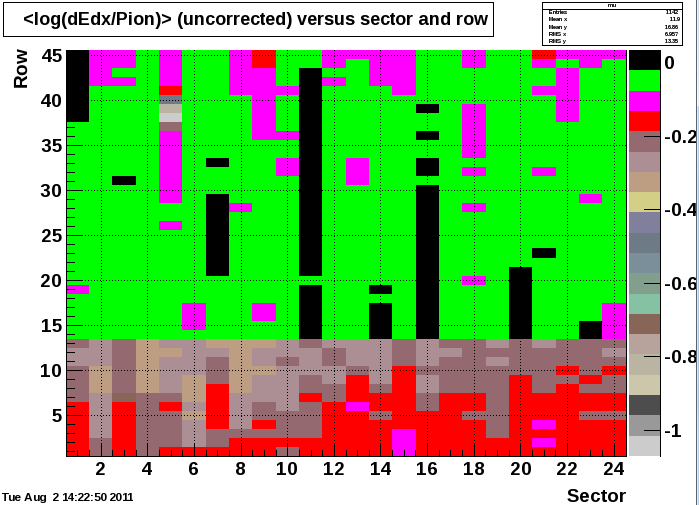
\includegraphics[width=0.4\textwidth]{fig/2.Detector/TPC/pass0_SectorRow}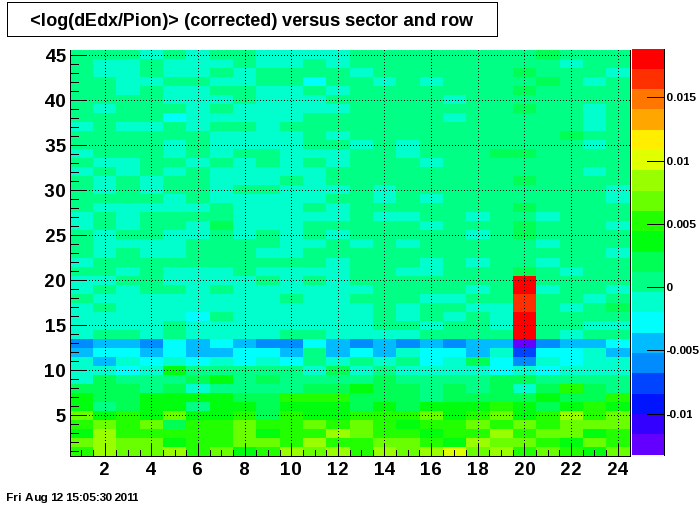
\includegraphics[width=0.4\textwidth]{fig/2.Detector/TPC/pass2_SecRow_mu}
\par\end{centering}

\protect\caption{Variation vs Sector and Row before SectorRow correction (left) and
after correction (right).}


\label{fig:SecRowCor}
\end{figure}


\begin{figure}
\begin{centering}
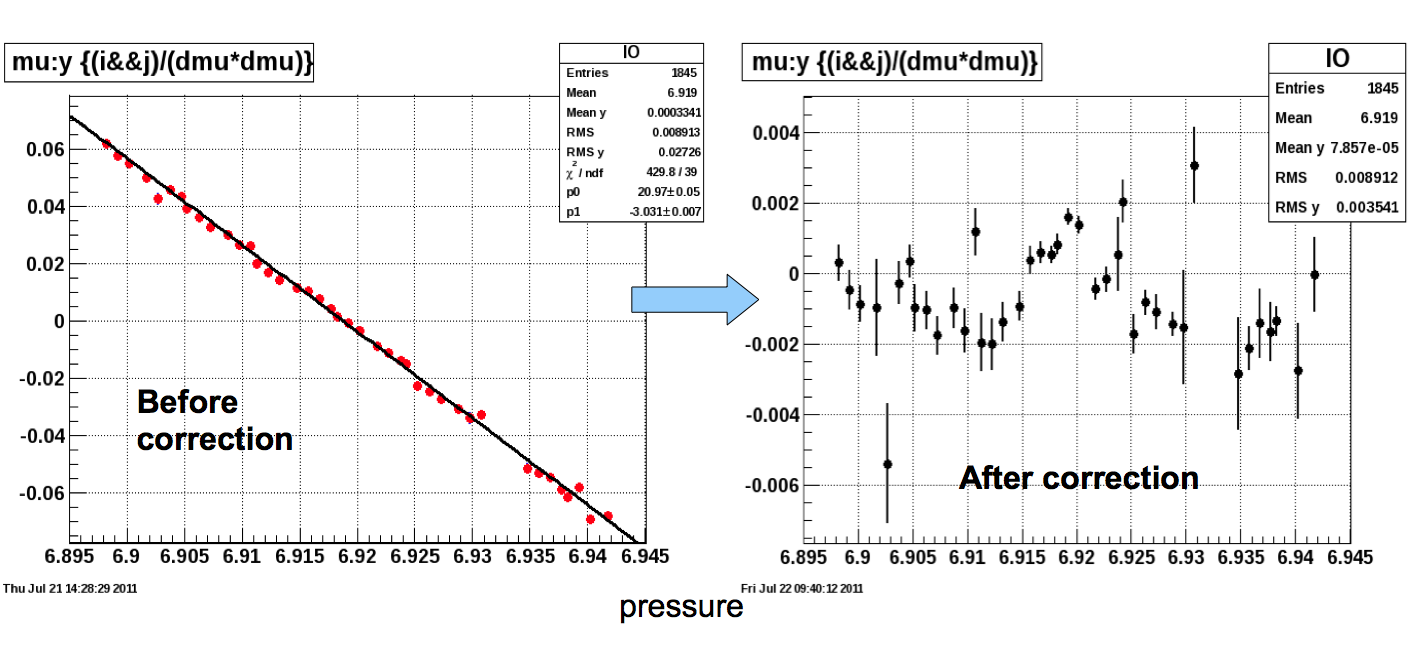
\includegraphics[width=0.8\textwidth]{/Users/luthien/Documents/Thesis/GitServer/Thesis/fig/2.Detector/TPC/PresureCor}
\par\end{centering}

\protect\caption{Variation vs gas pressure before correction (left) and after correction
(right).}


\label{fig:PresureCor}
\end{figure}


\begin{figure}
\begin{centering}
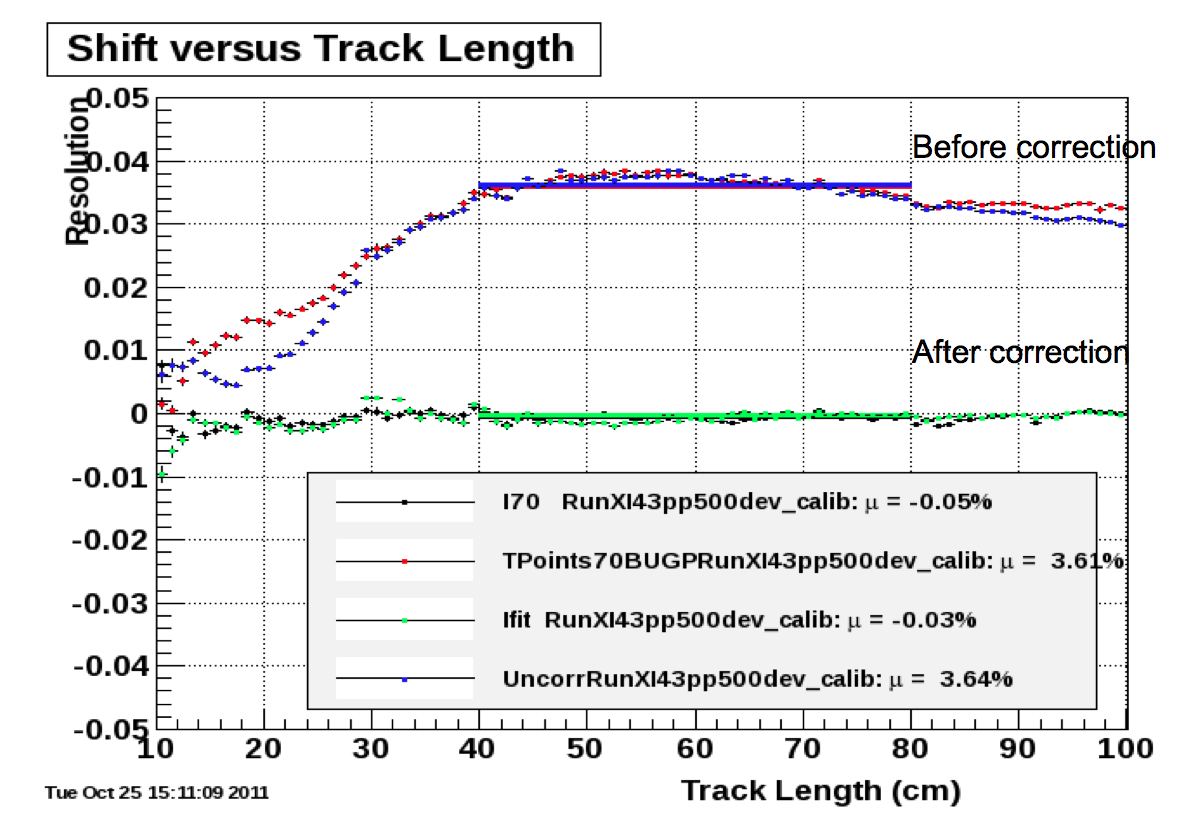
\includegraphics[width=0.8\textwidth]{fig/2.Detector/TPC/TrackLengthCor}
\par\end{centering}

\protect\caption{Variation vs track length before correction and after correction.}


\label{fig:TrackLengthCor}
\end{figure}


\begin{figure}
\begin{centering}
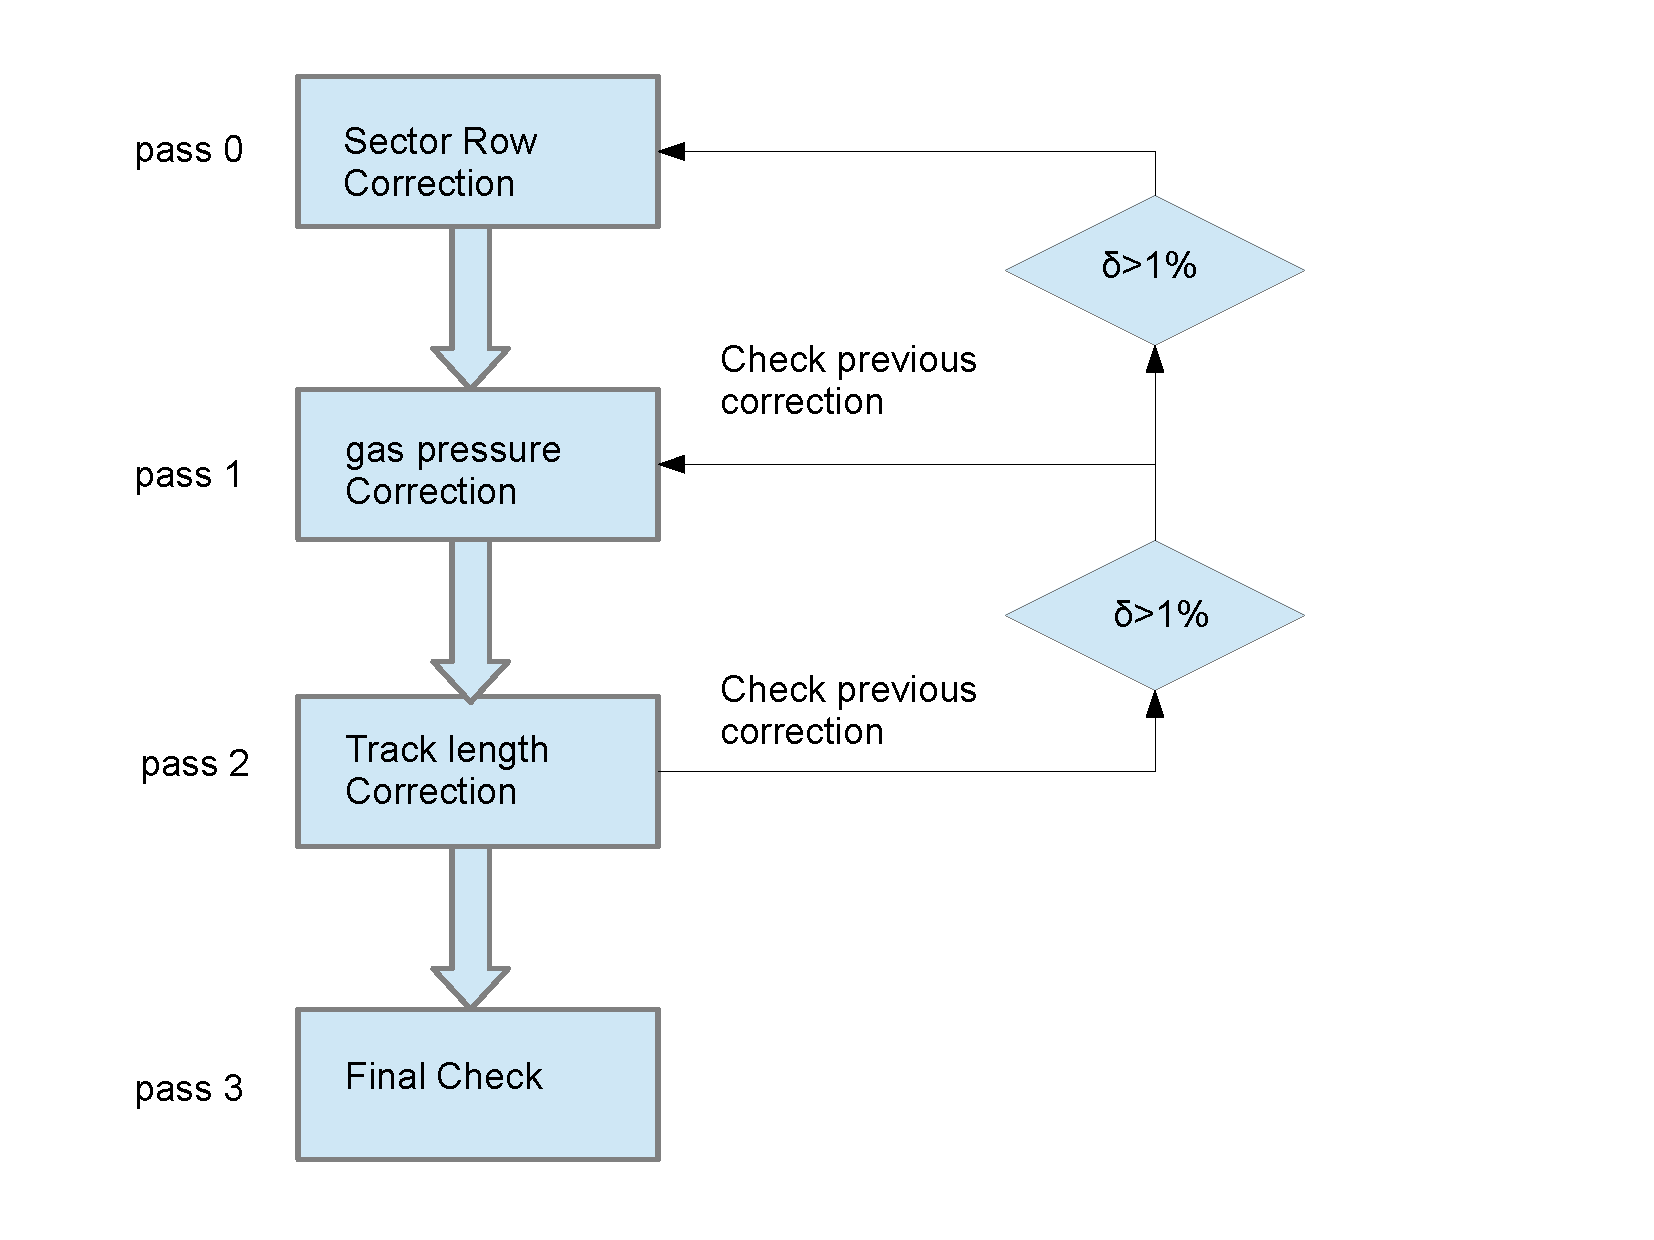
\includegraphics[width=0.8\textwidth]{fig/2.Detector/TPC/dEdx_Calib}
\par\end{centering}

\protect\caption{The procedure of\emph{ dE/dx }calibration. }


\label{fig:dEdx_Calib_procedure}
\end{figure}


\begin{figure}
\begin{centering}
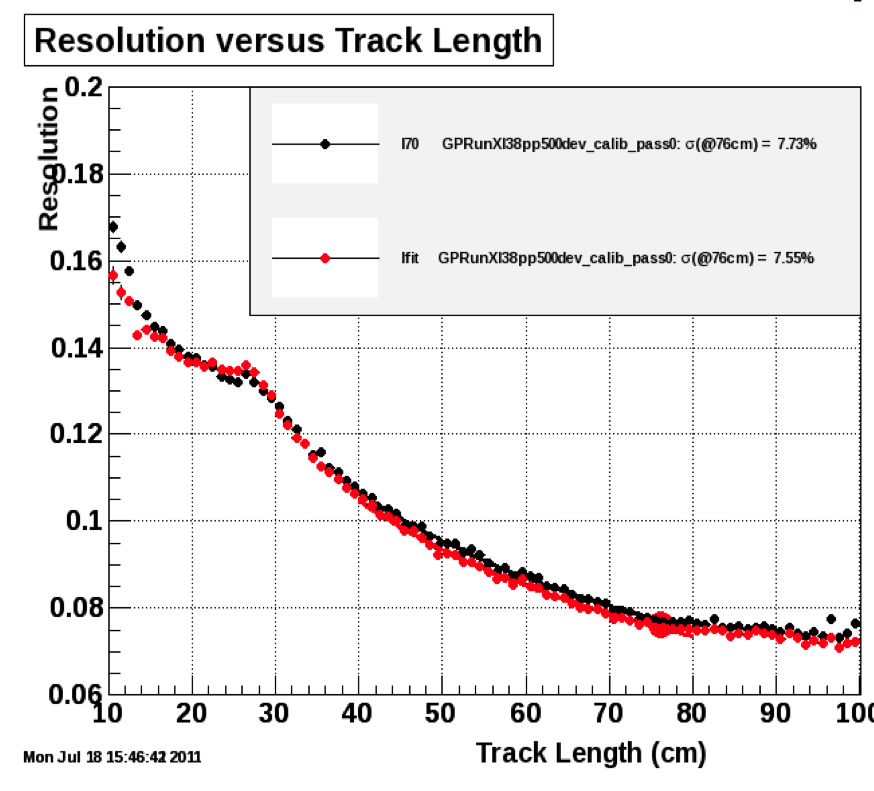
\includegraphics[width=0.4\textwidth]{fig/2.Detector/TPC/dEdxRes_pass0}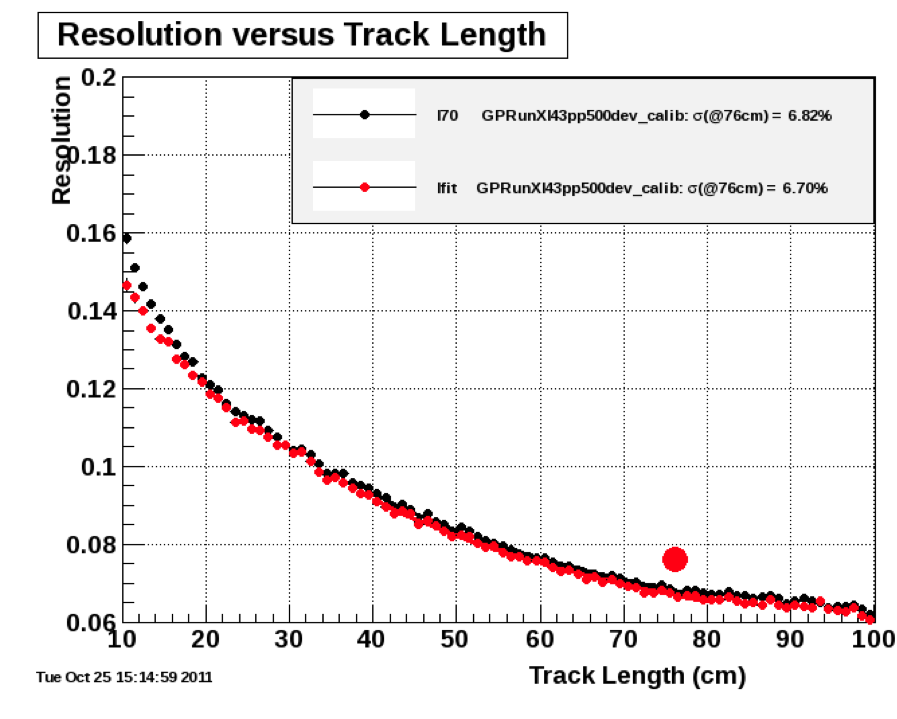
\includegraphics[width=0.4\textwidth]{fig/2.Detector/TPC/dEdxResPass3}
\par\end{centering}

\protect\caption{\emph{dE/dx} resolution as a function of track length without any
correction (left) and with all corrections (right) for p+p 500GeV
in Run11.}


\label{fig:dEdxRes}
\end{figure}



\subsection{Time Of Flight system}

The Time of Flight System (TOF) is another important set of detectors
used in this analysis. The TOF system is designed to measure the flight
time of charged particles. Combining with path length of tracks reconstructed
by TPC, it can provide the velocity of the charge particles which
is used to identify charged particles. In Fig. \ref{fig:dEdx_Bichsel},
the \emph{dE/dx} binds of different particles cross with each other
in some momentum regions where they can not be separated by using\emph{
dE/dx }only. With the installation of TOF, these holes are covered
by adding the flight velocity into the PID criteria. Therefore, TOF
greatly improves the PID capability of STAR and makes the identification
of electron and position from the hadron background possible for the
STAR detector system.

The TOF consists of the barrel Time Of Flight detector (bTOF) \cite{https://drupal.star.bnl.gov/STAR/files/future/proposals/tof-5-24-2004.pdf:kq}
and the the Vertex Position Detector (VPD). The bTOF is surrounding
the TPC and measures the ``stop'' time (the time charged particle
reach bTOF). The pVPD consists of two identical detector assemblies
that are positioned very close to the beam pipe and outside the STAR
magnet. It measures the start time (the time when the collision happens). 

The bTOF is based on the Multi-gap Resistive Plate Chamber (MRPC)
technology which is first developed by the CERN ALICE group \cite{CerronZeballos1996132}.
MRPC technology is capable to provide the necessary timing resolution
with a relative low cost. Figure \ref{fig:MRPC} shows the side view
of an MRPC module appropriate for STAR. Basically, the MRPC is a stack
of resistive plates arranged in parallel. These plates are separated
by nylon fishing line and form a series of uniform gas gaps with a
width of 0.22 mm. The internal resistive plates are 20 cm long and
6.1 cm wide and 0.54 mm thick, which has a resist of $8\times10^{12}\;\Omega\cdot cm$.
The external plates are $20.6\; cm\times7.6\; cm\times1.1\; mm$ with
electrodes on the outer surface. High voltage is applied on these
electrodes to generate a uniform strong electric field in each sub-gap.
All the internal plates are electrically floating. When charged particles
go through the chamber, they generates avalanches in the gas gaps.
The resistive plates are transparent to charge induction from avalanches
in the gaps. Thus the signal collected on the copper pickup pads is
the sum of possible avalanches from all gas gaps. The typical size
of a MRPC module is $94\: mm\times212\: mm\times12\; mm$ and the
active area is $61\; mm\times200\; mm$, and has 6 readout pads which
has an area of $63\; mm\times31.4\; mm$ with $3\; mm$ gaps between
pads.

One TOF tray consists of 32 MRPC modules which are installed alone
the beam direction. Every modules contains 6 read out units (cell/channel).
Figure \ref{fig:TOFTray} shows the structure of a STAR-TOF tray.
The bTOF contains 120 trays in total and has a coverage of $2\pi$
in azimuthal direction and $|\eta|<0.9$ in beam direction. The first
prototypes of TOF were installed in year 2003. 72\% of the bTOF were
installed in 2009 and fully installed with $2\pi$ azimuthal coverage
in 2010. The typical time resolution of TOF system is smaller than
100 ps. Figure \ref{fig:1/beta_TOF} shows the inverse velocity ($1/\beta$)
distribution as a function of momentum. With the installation of TOF,
the momentum range of separating $\pi$ and $k$ is improved from
0.7 GeV/c to 1.8 GeV/c, and proton identification range is improved
from 1.1 GeV/c to 3 GeV/c.

\begin{figure}
\begin{centering}
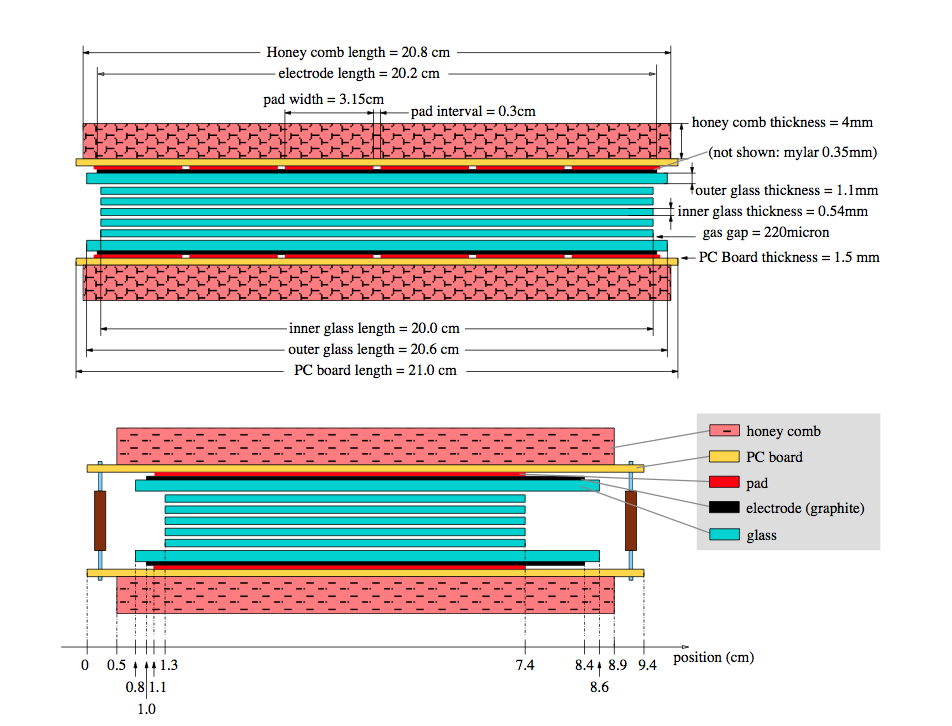
\includegraphics[width=0.9\textwidth]{fig/2.Detector/TOF/MRPC}
\par\end{centering}

\protect\caption{Two side views of the structure of an MRPC module. The upper (lower)
is for long (short) side view. The two plots are not at the same scale. }


\label{fig:MRPC}
\end{figure}
 

\begin{figure}
\begin{centering}
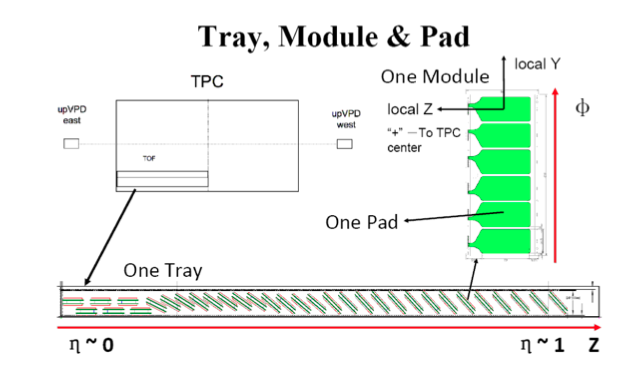
\includegraphics[width=0.8\textwidth]{fig/2.Detector/TOF/TrayModuleCell}
\par\end{centering}

\protect\caption{The structure of a STAR-TOF tray.}


\label{fig:TOFTray}
\end{figure}


\begin{figure}
\begin{centering}
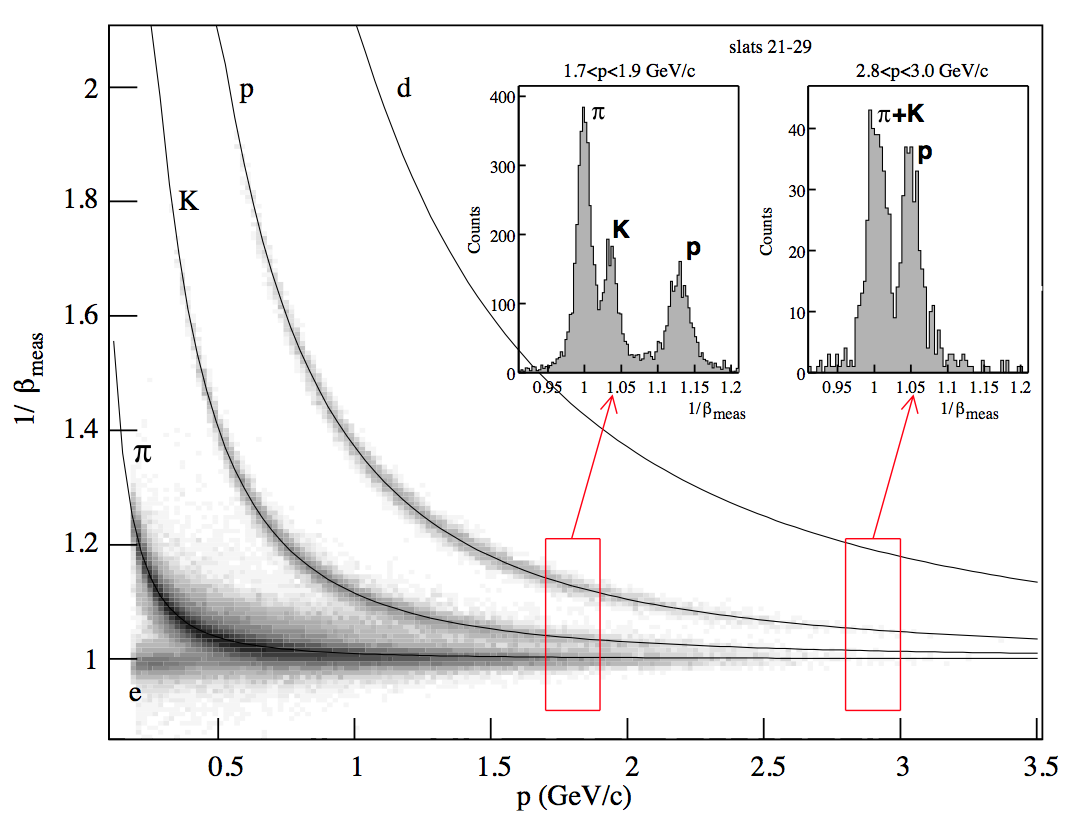
\includegraphics[width=0.8\textwidth]{fig/2.Detector/TOF/1overBeta_TOF}
\par\end{centering}

\protect\caption{$1/\beta$ vs momentum distributions. The solid lines show the expected
value for each particles}


\label{fig:1/beta_TOF}
\end{figure}



\subsection{STAR trigger system}

At STAR, the collision rate for Au+Au events is about 50 kHz, and
for high luminosity p+p collisions, this rate can reach up to 4MHz
which is close to the magnitude of the RHIC bunch crossing rate (10MHz).
However, the STAR DAQ system can only operate at a rate below 1800Hz
which is more than 3 magnitudes lower than the collision rate. Thus
a trigger system is needed to reduced the event rate. Furthermore,
only a small fraction of the collisions are physically interested.
The beam may hit residual gas atoms in the beam pipe and also beam
pipe itself, which makes a large fraction of the collisions are background.
These background events should be also suppressed by the trigger system.
The trigger system also includes triggers designed for special physics
purpose, such like, selecting events containing high $p_{T}$ particles
for heavy flavor and jet physics.

The STAR trigger system consist of three levels. Figure \ref{fig:TriggerDataFlow}
shows data flow through the trigger system. Level 0 examines every
branch crossing to determine whether there is a interested interaction
happened. It is constrained to issue a trigger decision within 1.5
$\mu s$ after the interaction. The signals from fast detectors are
digitized and sent into Data Storage and Manipulation (DSM) boards.
The DSM boards analyze these signals and form a decision tree which
is fead into Trigger Control Unit (TCU) board where the Level 0 trigger
decision is issued. Level 1 and 2 triggers apply more complex criteria
on events accepted by Level 0 trigger. Level 1 has a time budget \textasciitilde{}
100 $\mu s$ and Level 2 has about 5 ms. When an interaction is accepted
at Level 2, the trigger system notifies the DAQ system and detectors.
A review on the STAR trigger system can be find at \cite{Bieser2003766}.

\begin{figure}
\begin{centering}
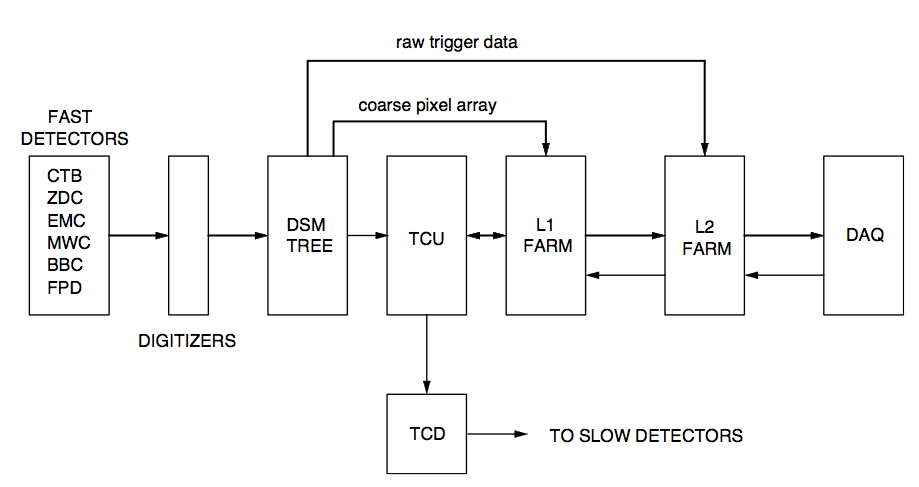
\includegraphics[width=0.8\textwidth]{fig/2.Detector/TriggerDataFlow}
\par\end{centering}

\protect\caption{Data flow through the trigger \cite{Bieser2003766}.}


\label{fig:TriggerDataFlow}
\end{figure}



\subsection{High Level Trigger/L4 system}

The High Level Trigger (HLT) system replaced the old Level 3 trigger
system which was abandoned since it could not catch up with STAR's
DAQ system upgrade. Similar with the old Level 3 trigger system, HLT
is trigger system base on online tracking and analysis. In Sec 2.2.4,
we introduced the multi-level trigger system based on fast hardwares
with simple trigger algorithms. It rejects most of the background
events and reduce the event rate down to a level under STAR DAQ system
limitation. At this points, for events selected by this trigger system,
signals from all detectors are digitized and passed to STAR DAQ system
for further processing. The HLT system is implemented after that.
Similar as the offline event reconstruction process, it collects informations
of subsystems from DAQ system, reconstructs events in real time, then
it issues a trigger decision base on real time PID and analyze. It
will select events with great physics interest, such as heavy fragmentation,
di-electrons, exotics and UPC collisions.

The prototype of STAR HLT was tested in 2009 and implied in 2010.
It worked as a tag system which tags events that pass through certain
analyze algorithm. During the RHIC Beam Energy Scan (BES) program,
it was used as an event monitor. Figure \ref{fig:HLT_old} shows the
architecture of the HLT system used during year 2009\textasciitilde{}2012.
It consists of two sub level, the Sector Level 3 (SL3) and the Global
Level three (GL3). SL3 shares half of the computing power on 24 TPX
computers, where cluster finding and track reconstruction are performed,
sector by sector. After that, tracks from all sectors as well as informations
from other subsystem are sent to GL3 machines, where they are assembled
and analyzed to make a real time event selection. Currently, BEMC
and TOF are included in HLT. 

\begin{figure}
\begin{centering}
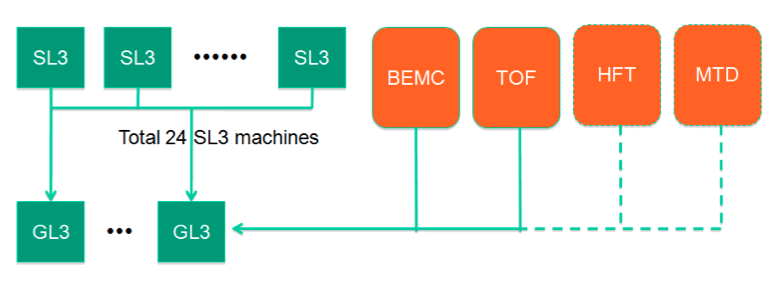
\includegraphics[width=0.8\textwidth]{/Users/luthien/Documents/Thesis/GitServer/Thesis/fig/2.Detector/HLT_old}
\par\end{centering}

\protect\caption{Architecture of the STAR high-level trigger. Solid lines connect the
currently used subsystems and dashed lines connect subsystems that
will be included in the future.}


\label{fig:HLT_old}
\end{figure}


To keep up with the speed of DAQ system, a few techniques and approach
have been implemented in HLT to increasing the processing speed. We
introduced the TPC hit map to combined the calculation and correction
for TPC hits in one step. It contains a grid map divided by all 24
sectors, all 45 pad rows, one for every 30 pads and one for every
40 time bucket. Points on the grid contains all the corrections the
same as offline reconstruction. Points between grids are calculated
as weighted average of adjacent grids. With the TPC hit map, the CPU
time of hits reconstruction is reduced from \textasciitilde{} 1 s
per event to \textasciitilde{}20 ms per event. Tracking reconstruction
in HLT is done sector by sector in parallel, so 24 times of speed-up
is naturally achieved. The STAR HLT tracker is based on conformal
mapping \cite{Adler2003778} and a follow-your-nose approach on finding
next-hit-on-track. These approaches greatly reduces the track time
with little loss on efficiency and track resolution (at $p_{T}$>1
GeV/c efficiency w.r.t offline is 90\% and momentum difference w.r.t
offline is less than 2\%). The TOF and BEMC calibration tables for
HLT was made following the same procedure as offline. The EMC pedestal
and gain table are the same as the one used by STAR's lower level
triggers. The TPC \emph{dE/dx }calibration is made by adjusting the
\emph{dE/dx }gain obtained from the previous run, for inner and outer
sector separately. The calibration for TPC hit positions are folded
into the TPC hit map based on offline calibration tables.

During year from 2010 to 2012, the STAR HLT has delivered several
important physics results by selecting events containing heavy fragments,
di-electrons and high $p_{T}$ tracks. It played a very important
role in the finding $\bar{^{4}He}$ in $\sqrt{s_{NN}}$ = 200 GeV
Au+Au collisions by triggering on events containing charge-2 particles.
This discovery has been published in \emph{Nature \cite{:2011qf}.
}A brief review about the HLT and its future development can be find
at \cite{Ke:2013uq}.


\section{Future upgrade}

In 2014, two new detectors was added into the STAR detector system.
Installed in the most outside of STAR is the Muon Telescope Detector
(MTD), which is a $\mu$ detector. MTD is based on long-MRPC technology,
covers 45\% acceptance ($|\eta|<0.5$) in $\eta$ direction and $2\pi$
in azimuthal direction. It uses the BEMC and the magnet steel as the
absorber of electrons and hadrons. The first prototype was installed
in STAR in year 2007, and showed good performance in the following
runs. In 2014, MTD has been fully installed and significant data set
was taken with it. Another detector installed in 2014 is Heavy Flavor
Tracker (HFT). The HFT is an inner vertex detector which was installed
between the beam pipe and TPC. It consists of two layers of pixels
located at mean radius of 1.5 cm and 5 cm from the center of beam
pipe and the Silicon Strip Detectors (SSD) to fill the gap between
the innermost pixel detector and the TPC. 
